\documentclass{chi-ext}
% Please be sure that you have the dependencies (i.e., additional LaTeX packages) to compile this example.
% See http://personales.upv.es/luileito/chiext/

\copyrightinfo{
  Copyright is held by the author/owner(s).\\
  \emph{CHI'13}, April 27 -- May 2, 2013, Paris, France.\\
  ACM 978-1-XXXX-XXXX-X/XX/XX.\\
}

\title{Using Distributed Information Stores for Patient-Clinician Health Data Sharing}

\numberofauthors{3}
% Notice how author names are alternately typesetted to appear ordered in 2-column format;
% i.e., the first 4 autors on the first column and the other 4 auhors on the second column.
% Actually, it's up to you to strictly adhere to this author notation.
\author{
  \vspace{-1.5em} % lisatolles: The abstract heading should start at the time height on the page as the authors names
  \alignauthor{
  	\textbf{Daniel A. Smith}\\
  	\affaddr{Web and Internet Science Research Group}\\
%  	\affaddr{Electronics and Computer Science}\\
  	\affaddr{University of Southampton}\\
  	\affaddr{Southampton, UK}\\
  	\email{ds@ecs.soton.ac.uk}
  }\alignauthor{
  	\textbf{Max Van Kleek}\\
  	\affaddr{Web and Internet Science Research Group}\\
%  	\affaddr{Electronics and Computer Science}\\
  	\affaddr{University of Southampton}\\
  	\affaddr{Southampton, UK}\\
  	\email{emax@ecs.soton.ac.uk}
  }
  \vfil
  \alignauthor{
  	\textbf{Nigel R. Shadbolt}\\
  	\affaddr{Web and Internet Science Research Group}\\
%  	\affaddr{Electronics and Computer Science}\\
  	\affaddr{University of Southampton}\\
  	\affaddr{Southampton, UK}\\
  	\email{nrs@ecs.soton.ac.uk}
  }
  \vfil
  \vfil
  \vfil
  \vfil
}

% Paper metadata (use plain text, for PDF inclusion and later re-using, if desired)
\def\plaintitle{Using Distributed Information Stores for Patient-Clinician Health Data Sharing}
\def\plainauthor{Daniel A. Smith, Max Van Kleek, Nigel R. Shadbolt}
\def\plainkeywords{personal data, patient care, healthcare, information stores}
\def\plaingeneralterms{Personal Data, Patient Care, Healthcare, Information Stores}

\hypersetup{
  % Your metadata go here
  pdftitle={\plaintitle},
  pdfauthor={\plainauthor},  
  pdfkeywords={\plainkeywords},
  pdfsubject={\plaingeneralterms},
  % Quick access to color overriding:
  %citecolor=black,
  %linkcolor=black,
  %menucolor=black,
  %urlcolor=black,
}


\usepackage{graphicx}   % for EPS use the graphics package instead
\usepackage{balance}    % useful for balancing the last columns
\usepackage{bibspacing} % save vertical space in references

\usepackage{url}

\begin{document}

\maketitle

\begin{abstract}

Existing approaches to electronic integrated health records have largely focused on centralised information architectures, where patient data is held in a single repository, and accessed over the internet. However, there are a number of benefits to both patients and clinicians in a decentralised information approach to health records.

\end{abstract}

\keywords{\plainkeywords}
%\textcolor{red}{Mandatory section to be included in your final version.}

\category{H.5.m}{Information interfaces and presentation (e.g., HCI)}{Miscellaneous}. 
%See \cite{ACMCCS} 
%See: \url{http://www.acm.org/about/class/1998/} 
%or help using the ACM Classification system.
%\textcolor{red}{Mandatory section to be included in your final version.}

%\terms{\plaingeneralterms}
%\textcolor{red}{Optional section to be included in your final version.}


\section{Introduction}
A key goal in improving patient-clinician communication is
establishing a common context for communication with which a shared
understanding can be established.  This understanding is
bi-directional, in the sense that the patient needs to be able to
effectively interpret what the clinician is trying to convey to him or
her, but also that the clinician needs to be able to arrive at an
accurate characterisation of the patient's situation and condition, as
updated since the patient was last seen. This is often under time
pressure and with limited access to information about how the patient
has been in the interim.

One of the most promising technologies that has the potential to help
provide such a common context is the patient-centric electronic health
record (henceforth EHR)\cite{hayrinen2008definition}, a digital representation of the
complete medical history of an individual as recorded by clinicians
throughout a patient's life. The EHR has enabled both patients and
their clinicians unfettered access to the patient's medical data,
including diagnostics, reports, and history of interventions.  This
means that clinicians can more easily review a patient's long-term
history even under time pressure and constraints. Moreover, since
patients have access to their own medical histories, they can access
the raw information that was the basis for a prognosis or decision.

% proactive activity recording to provide sketches of a person's
% activity profiles outside of the hospital, streaming data

\marginpar{
\begin{figure}
  \hspace{-11mm}
  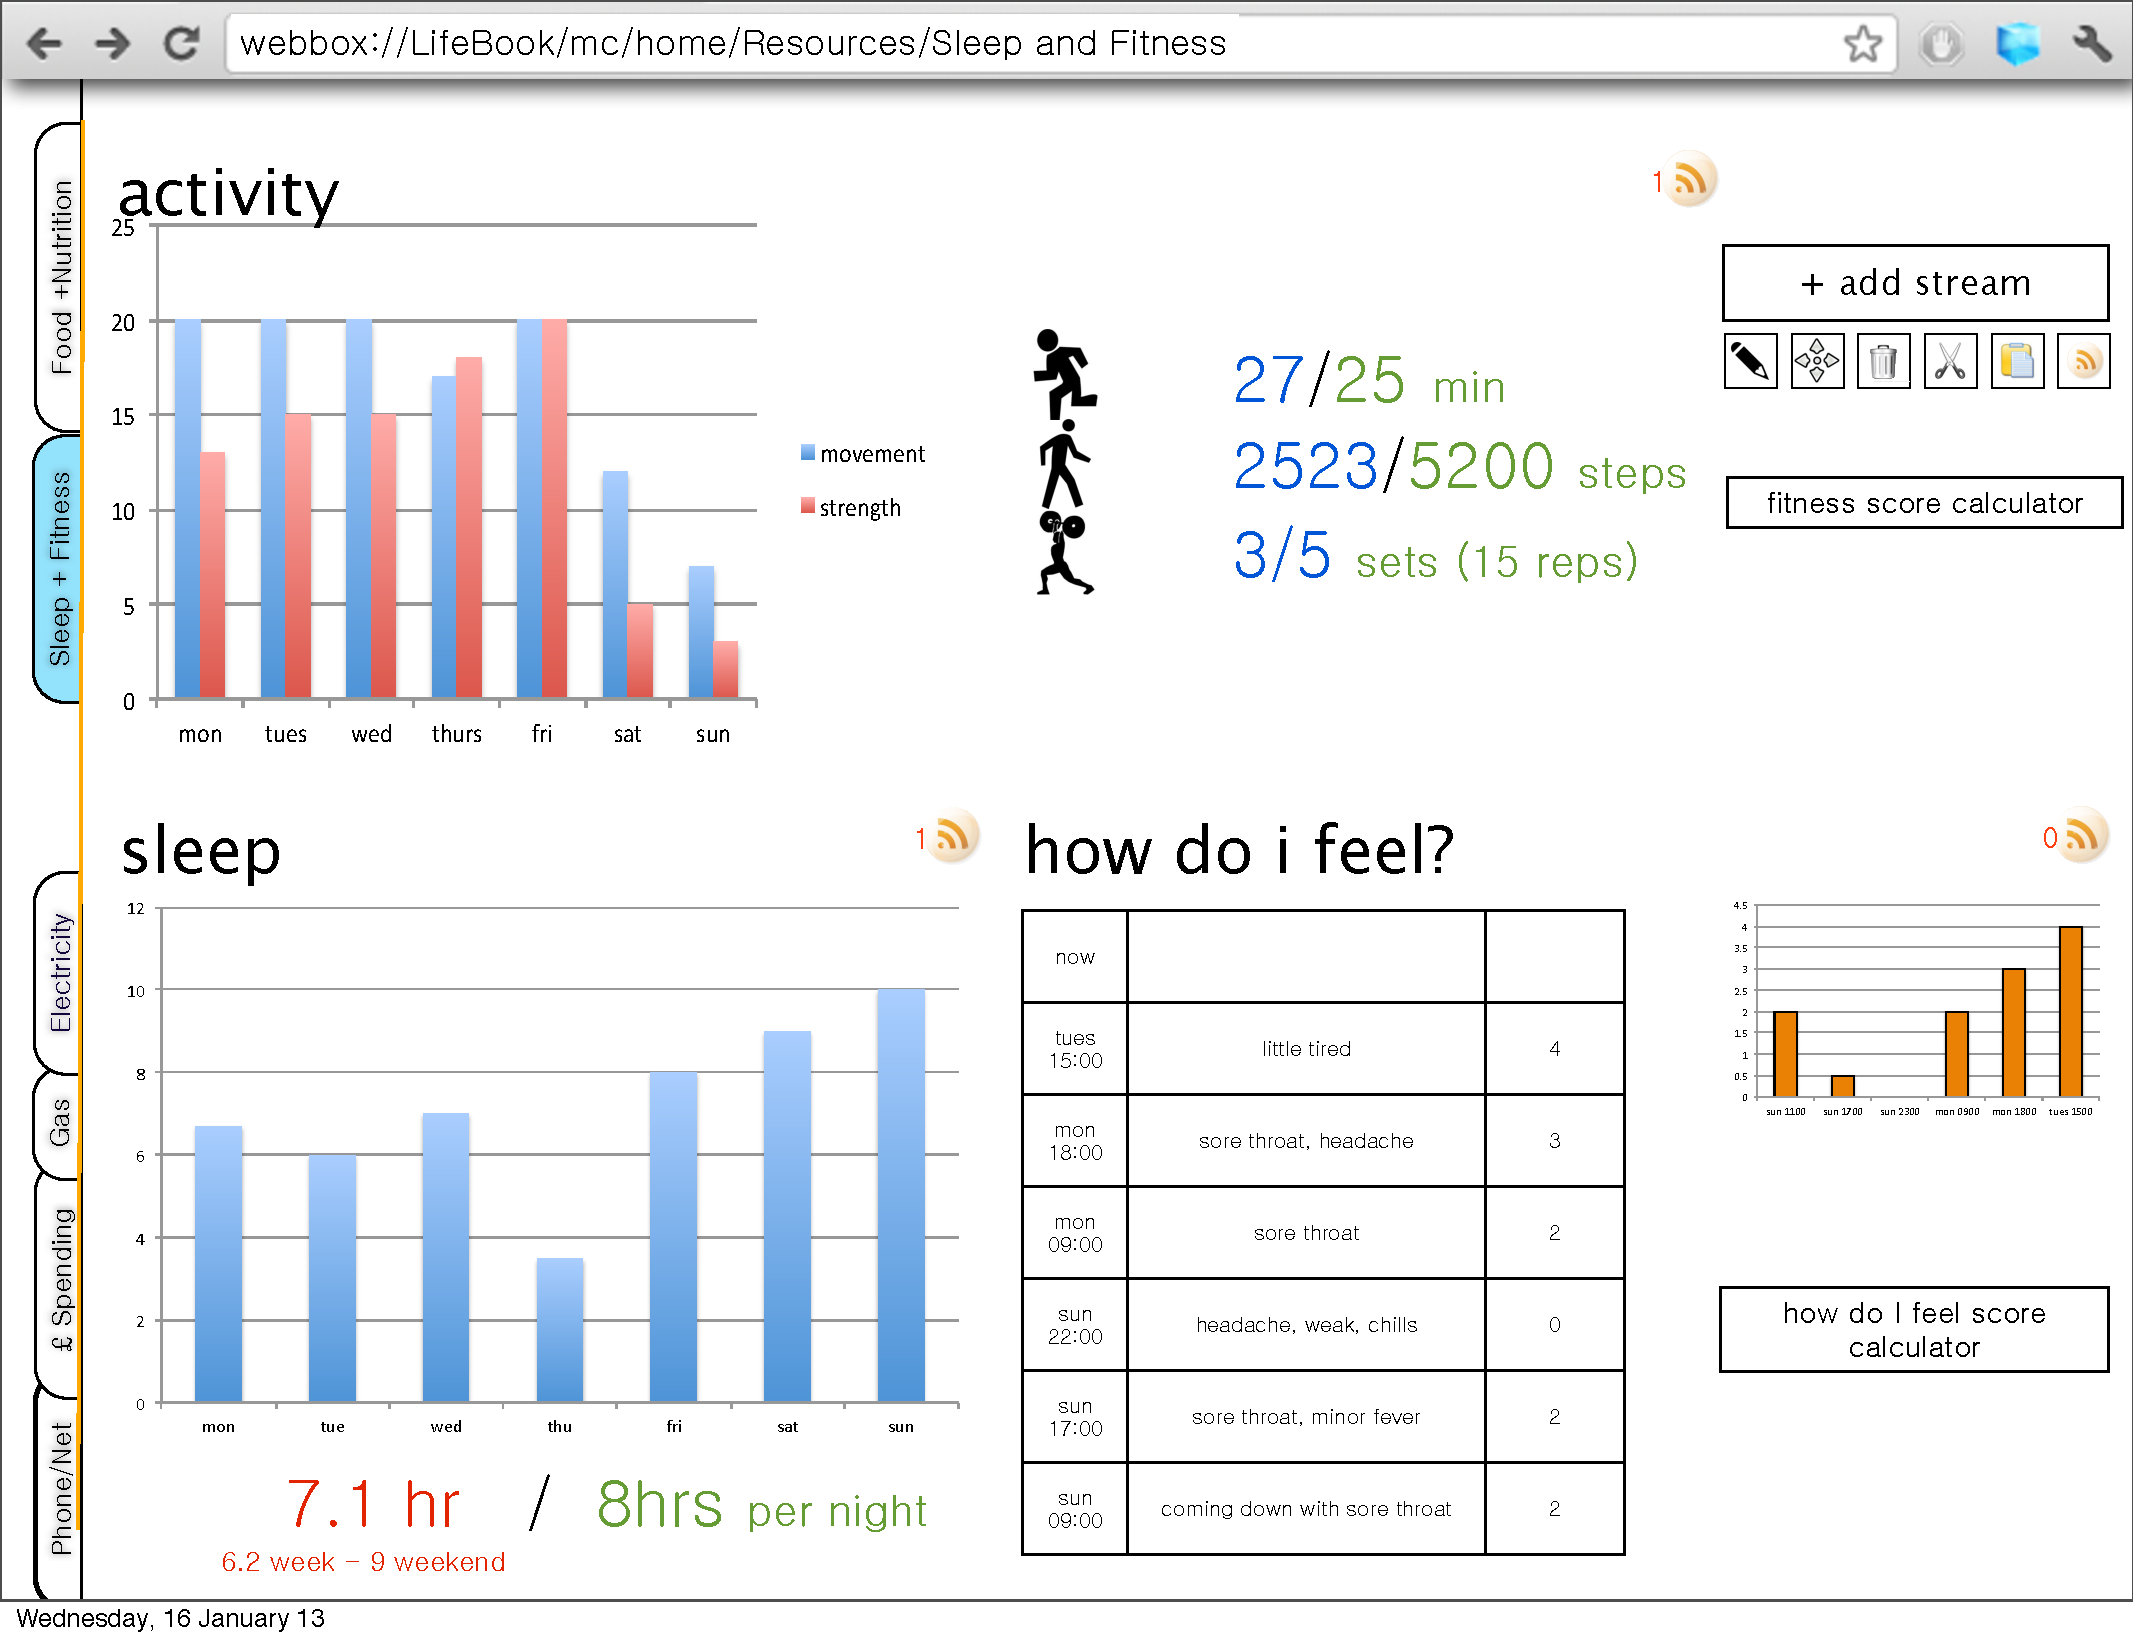
\includegraphics[width=5.5cm]{img/energy-scenario}
  \caption{Mock-up of an activity diary dashboard, showing data from multiple devices.}
  \label{fig:mockup}
\end{figure}
}



Yet, so far, EHRs have primarily been limited to the storage of
official diagnostic reports prepared by clinicians, technicians and
nurses.  These communications are both highly technical, making them
difficult to interpret by end-user patients, but also highly limited
in temporal resolution, reflecting only cases where a person was
attended to and diagnostic-tested by a medical professional.  Although
this may be frequent for patients in inpatient care, those that come
to see their clinician, say, once a month end up with extremely
low-resolution samples of a patient's condition.

In this position paper, we look at the potential and problems of
augmenting the next generation of EHRs with \emph{personal activity
  diaries}, portraits of a person's dynamic condition captured at high
temporal fidelity.  Such activity diaries are intended to supplement,
rather than supplant, the existing diagnostic reports performed by
professionals, first and foremost, to help clinicians derive a more
complete picture of the person throughout a period of care, such as an
intervention.  We believe that such activity diaries could potentially
also be beneficial to individuals as well, making people more aware of
the evolution of their health.

Nonetheless, challenges abound. These primarily pertain to capturing
these activity diaries, effectively storing these diaries, giving
users easy-to-use access to these diaries, and privacy controls for
giving patients the ability to disclose desired quantities of their
diary to their clinicians.  We discuss these, next.

\section{Using activity diaries}

We imagine integrated activity diaries to be used by both clinicans
and patients in several ways.  First, for nearly all types of
conditions, monitoring a person's overall daily activity and sleep
duration could easily indicate how much rest, exercise, exposure to
others, and the outside world he or she might be getting.  Daily
records of the time(s) that a person gets up, eats, works, exercises
and relaxes can be analysed by clincians for irregular behaviours or
habits that might be affecting a person's well-being. For more
specific conditions, daily measurements of a person's blood pressure,
blood oxidation, heart rate, breathing, weight, and galvanic skin
response could be useful for tracking progress on a prescribed
intervention, recovery from an illness, or onset of a new conditions,
for example, or be used to pinpoint sources of prolonged stress.

Merely providing access to such activity records back to individuals
could have direct effects on people's behavior, motivation and
perceived well-being.  For example, just as asking individuals to
introspect and justify their opinions and feelings has been found to
be both disruptive and reinforcing of their opinions
\cite{wilson1989introspection}, allowing people to reflect upon their
historical records of their activities might help people realize or
change their minds about how or why they feel particular ways. We feel
that there is significant room for investigation here, and potential
for research pertaining to self motivation and improvement.

\marginpar{
\begin{table}
\small
\vspace{0.5cm}
\begin{tabular}{p{3cm}  p{6cm} p{1.5cm}}

product & measurement indices & price range (approx. USD) \\
\hline
FitBit & general activity (walking/jogging) & \$50 \\
Nike FuelBand & general activity (walking/jogging) & \$199 \\ 
Writhings WiFi Scale & weight & \$200 \\
Writhings BPM & blood pressure & \$200 \\ 
Zeo Pro & sleep duration \& quality & \$200 \\
WakeMate & sleep duration & \$50  \\
Zensorium Tinkne & heart rate variability, blood oxygenation, respiratory rate & \$200 \\
BodyMedia CORE 2 & galvanic skin repsonse, body temperature, sleep, respiratory rate, heart rate & (TBD) \\
Hapifork & eating time, rate, frequency & (TBD) \\ 
\end{tabular}
\caption{\emph{Consumer-grade activity sensors}: Activity and physiological measurememnt sensors with automatic data uplink to cloud services }
\label{sensors}
\end{table}
}
\vspace{6cm}

\section{Capturing activity diaries}

The recent proliferation in personal wearable activity sensors and
network and storage- enabled digital health measurement devices has
been driven by both the falling costs of embeddable electronics, and a
surging public interest in ``quantified-self''-style self-monitoring
for self-improvement.  Many of these sensors are lightweight, can be
worn discreetly, measure several physiological statistics
simultaneously, and most require little maintenance. Table
\ref{sensors} lists a variety of such sensors, currently available
readily from online retailers.

While few of these devices had been independently evaluated for
accuracy for clinical use, as they have matured, several of these
manufacturers begun rigorous evaluaton of their products for achieving
certification. For example, BodyMedia advertise themselves as
providing the ``FDA-approved, clincally validated, most accurate
wireless activity measurement''.  A separate study of activity-based
sleep monitoring tools revealed that ``low cost actigraphy-based
approaches'' correlated well with baseline (in-lab EEG-based
measurements) for sleep duration, although less with sleep quality
metrics.

%% In addition to fitness monitors, the market for quantified self sensors has
%% expanded into areas of personal health. For example, there are sensors for
%% measuring blood oxygenation\footnote{SpO2 Blood Oxygenation sensor: \url{http://ispo2.com}},
%% Heart Rate Variability and Respiratory Rate\footnote{Zensorium Tinke, heart and respiratory rate sensor: \newline \indent \indent \indent \url{http://www.zensorium.com/tinke/}} and
%% Temperature and Galvanic Skin Response\footnote{BodyMedia Core 2, temperature and GSR sensor: \newline \indent \indent \indent  \url{http://www.bodymedia.com}}.
%% The diet aspect of weight loss is also covered, by products such as a wireless fork that informs you how long you spent eating\footnote{HapiLabs HapiFork: \newline \indent \indent \indent  \url{http://hapilabs.com/products-hapifork.asp}}.


\section{Storing and Representing Activity Diaries}

Currently, these products are designed to work separately by themselves, uploading sensor measurements to dedicated web sites set up by each device's manufacturer.  Such sites are poorly suited for the long-term storage for the highly personal activity data for several reasons; first, none of the sites provide any long-term retention or access guarantees of user data (nor HIPAA security guarantees).  Second, it is difficult for a user to gain a unified understanding of their activity across their devices through the disparate interfaces provided by these services, due of the widely different visual and interface representations provided. Finally, many of these visualisations represent user activity in arbitrary, ``user-friendly'' units, such as ``Sleep score'', ``Fuel'', ``Zen level'', which, being not rigorously defined are difficult or impossible to compare across services.

However, many of these sites have APIs that provide access to the raw sensor data, making it feasible to access and interpret captured data.  We propose that these APIs be used to consolidate information from among all of the services corresponding to a patient's personal health devices, into a single representation kept with their EHR.  In particular, grounding this activity data in a uniform, common taxonomy and description logic, like those provided for medical diagnoses and diseases through SNOMED-CT \cite{stearns2001snomed} and ICD-10 \cite{world1993icd}, would enable these diaries to interpretable by future clinical medical systems, such as primary care information management systems. 

Since SNOWMED-CT nor ICD cover routine measured activity, we are devising a supplemental ontology for these concepts called \emph{Activity-SENSE}.  This ontology encompasses patient activities, and standard units of measure with which activities are measured, as well as the ability to describe the sensors used.  The intention is for Activity-SENSE records to, like those of SNOMED-CT, eventually be translatable to different languages and mapped to other similar ontologies of behaviour.

\section{The WebBox EHR Platform}

The high-resolution data collected by activity-sensing devices, accumulated over a long period such as a patient's lifespan, can result in a substantially greater volume of data than current EHR platforms are designed to handle. To address this deficiency, we have devised a personal data platform ``WebBox \cite{webbox}'', optimised to handle the secure, long-term storage of structured data at large volume.  Thus far, WebBox has been used to archive clinician (hospital and GP-provided) data, including both raw structured data (such as clinical diagnostic results) and traditional reports prepared by clinicians.  Being optimised for structured data capture and integration, our current work extends this platform to the aforementioned activity profiles, created from retrieving raw sensed data from digital health device APIs and translating such observations to the Activity-SENSE representation.  

%Following this, to optionally share these annotations, along with their activity diaries, with their clinician. This then enables clinicians and patients to enter into a dialog about how well the patient is doing, and any lifestyle changes they can make to better their situation.


%% Furthermore, Therefore, existing platforms for storing EHRs may
%% prove to be unsuitable for the large volumes of data from activity diaries. However, integrating with existing EHRs
%% would enable clinicians and patients to view the data in context. 


%% Such a representation might enable GPs to more quickly understand a   such as for providing
%% like the SNOWMEDif Building such a representation, however, makes several assumptions, the 
%%   We propose that   to be harvested and stored into unified representations, such as to be stored with a person's 
%%   single product are peruploaded by the devices to 
%% are presented either on the device themselves, or via a smartphone or website. However,
%% their use could be integrated with clinical care, in order to monitor patients, and to give an
%% insight into their lifestyle.

%% In order to do this, the data from each device should be collected and archived, so it can
%% be viewed together in an appropriate interface. The data collected by patients' devices has
%% the potential to create a large volume of data, and therefore particular
%% consideration should be paid about who and where the data will be stored. In particular, it is likely
%% that existing providers of storage for electronic health records will not want to be burdened with the
%% administration costs of storing additional data. The longevity of third-party storage providers is
%% also a concern, because there has b een a history of short-notice closures of EHR providers (such as Google Health).


%Particular care should be taken when deciding on a format to store the activity diaries. Ideally
%a format will be machine-readable, using open standards (for example XML, RDF or JSON) and
%following existing schematic/ontological knowledge modelling conventions. There are a 
%number of medical ontologies that already exist, as well as vocabularies and systems (such as
%SNOMED CT \cite{stearns2001snomed} and IDC-10) that focus on the medical domain. The hope is that by using
%such systems, that the data collected by patients can be analysed more rapidly by clinical systems
%and staff.
%
%One option is to embrace the Semantic Web, because it offers several key benefits:
%
%\begin{itemize}
%
%\item Distributed system with universal addresses and standard mature protocols
%\item Open extensible ontology system and existing domain ontologies
%\item Existing library and tool support and expertise
%\item Interoperability with existing systems
%
%\end{itemize}
% 
%Even if personal health records or systems do not use the Semantic Web, there are existing
%techniques to integrate with their data.

%% \section{Privacy Controls}

%% One of the major concerns with storage of patient data is privacy. Indeed, there is also potentially
%% legal requirements on storing personal health data, depending on the nature of the data being
%% stored.

%% However, it is important that control of data be sufficiently granular so that patients can choose
%% to sure it with clinicians, and that clinicians can refer to it in their notes in the patient's health
%% record.


%% \section{Conclusion}

%% By augmenting data from personal health sensors with EHRs, both patients and clinicians
%% can gain insight into the lifestyle and typical activities of a patient. Challenges in implementation
%% of such a system do exist, but through the use of domain ontologies and peer-to-peer
%% sharing...



\section{Biographies}

\subsection{Daniel A. Smith and Max Van Kleek}

Daniel and Max are postdoctoral researchers on the SOCIAM project at the University of Southampton, and the principal architects of the WebBox
personal information store. They have research interests in HCI, the Semantic Web and Personal Information Management.


\subsection{Nigel R. Shadbolt}

Nigel Shadbolt (FBCS FREng) is Professor of Artificial Intelligence and Head of the Web and Internet Science Group, University of Southampton. He is the Chairman and Co-Founder of the Open Data Institute, Director of the Web Science Trust, and the Web Foundation.  He is a member of the Public Sector Transparency Board, and Chair of the UK Government's midata programme. He and Sir Tim Berners-Lee are Information Advisors to the UK Government, responsible for \url{data.gov.uk}, which has released thousands of NHS health data sets.



%% \section{Key Technology: WebBox}

%% WebBox is...


\section{Acknowledgement}

This work is supported by the SOCIAM Project (EPSRC grant EP/J017728/1).



%% =============================================================================
%\section{Introduction}
%% =============================================================================
%This format is to be used for submissions that are published in the conference extended abstracts.  
%We wish to give this volume a consistent, high-quality appearance. 
%We therefore ask that authors follow some simple guidelines. 
%In essence, you should format your paper exactly like this document. 
%The easiest way to do this is simply to download a template from the conference website and replace the content with your own material.
%
%% =============================================================================
%\section{Copyright}
%% =============================================================================
%For publications in the CHI Extended Abstracts, copyright remains with the author.  
%The publication is not considered an archival publication; however, it does go into the ACM Digital Library. 
%Because you retain copyright, as the author you are free to use this material as you like, including submitting a paper based on this work to other conferences or journals.  
%Authors grant unrestricted permission for ACM to publish the accepted submission in the CHI Extended Abstracts without additional consideration or remuneration.
%
%% =============================================================================
%\section{Text formatting}
%% =============================================================================
%Please use an 8.5-point Verdana font, or other sans serifs font as close as possible in appearance to Verdana in which these guidelines have been set. 
%Arial 9-point font is a reasonable substitute for Verdana as it has a similar x-height. 
%Please use serif or non-proportional fonts only for special purposes, such as distinguishing source code text.
%Additionally, here is an example of footnoted text.\footnote{Use footnotes sparingly, if at all.}
%As stated in the footnote, footnotes should rarely be used.
%
%\subsection{Language, style, and content}
%% -----------------------------------------------------------------------------
%The written and spoken language of SIGCHI is English. 
%Spelling and punctuation may use any dialect of English (e.g., British, Canadian, US, etc.) provided this is done consistently. 
%Hyphenation is optional. 
%To ensure suitability for an international audience, please pay attention to the following:
%
%\begin{itemize}\compresslist
%\item 	
%Write in a straightforward style. 
%Use simple sentence structure. 
%Try to avoid long sentences and complex sentence structures. 
%Use semicolons carefully.
%\item 	
%Use common and basic vocabulary (e.g., use the word ``unusual" rather than the word ``arcane").
%\item 	
%Briefly define or explain all technical terms. 
%The terminology common to your practice/discipline may be different in other design practices/disciplines.
%\item 	
%Spell out all acronyms the first time they are used in your text. 
%For example, ``World Wide Web (WWW)".
%\item 	
%Explain local references (e.g., not everyone knows all city names in a particular country).
%\item 	
%Explain ``insider" comments. 
%Ensure that your whole audience understands any reference whose meaning you do not describe (e.g., do not assume that everyone has used a Macintosh or a particular application).
%\item 	
%Explain colloquial language and puns. 
%Understanding phrases like ``red herring" requires a cultural knowledge of English. 
%Humor and irony are difficult to translate.
%\item 	
%Use unambiguous forms for culturally localized concepts, such as times, dates, currencies and numbers (e.g., ``1-5-97" or ``5/1/97" may mean 5 January or 1 May, and ``seven o'clock" may mean 7:00 am or 19:00).
%\item 	
%Be careful with the use of gender-specific pronouns (he, she) and other gender-specific words (chairman, manpower, man-months). 
%Use inclusive language (e.g., she or he, they, chair, staff, staff-hours, person-years) that is gender-neutral. 
%If necessary, you may be able to use ``he" and ``she" in alternating sentences, so that the two genders occur equally often~\cite{Schwartz95}. 
%\end{itemize}
%
%
%% =============================================================================
%\section{Figures}
%% =============================================================================
%The examples on this and following pages should help you get a feel for how screen-shots and other figures should be placed in the template. 
%Be sure to make images large enough so the important details are legible and clear.
%
%%\begin{figure}
%%  \centering
%%  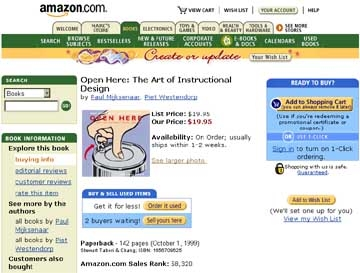
\includegraphics[width=\linewidth]{sample.jpg}
%%  \caption{Insert a caption below each figure.}
%%  \label{fig:sample}
%%\end{figure}
%
%Your document may use color figures, which are included in the page limit; the figures must be usable when printed in black and white.
%You can use the \LaTeX's \texttt{marginpar} command to insert figures in the (right) margin side of the document (see \autoref{fig:marginparsample}).
%
%
%% =============================================================================
%\section{References and Citations}
%% =============================================================================
%Use a numbered list of references at the end of the article, ordered alphabetically by first author, and referenced by numbers in brackets \cite{Anderson92,Klemmer02,Mather00,Zellweger01}
%For papers from conference proceedings, include the title of the paper and an abbreviated name of the conference (e.g., for Interact 2003 proceedings, use Proc. Interact 2003). 
%Do not include the location of the conference or the exact date; do include the page numbers if available. 
%See the examples of citations at the end of this document. 
%
%Your references should be published materials accessible to the public.  
%Internal technical reports may be cited only if they are easily accessible (i.e., you provide the address for obtaining the report within your citation) and may be obtained by any reader for a nominal fee.  
%Proprietary information may not be cited. 
%Private communications should be acknowledged in the main text, not referenced  (e.g., [Robertson, personal communication]).
%
%
%% =============================================================================
%\section{Producing and testing PDF files}
%% =============================================================================
%We recommend that you produce a PDF version of your submission well before the final deadline. 
%Besides making sure that you are able to produce a PDF, you will need to check that (a) the length of the file remains within the submission category's page limit, (b) the PDF file size is 4 megabytes or less, and (c) the file can be read and printed using Adobe Acrobat Reader. 
%Test your PDF file by viewing or printing it with the same software we will use when we receive it, Adobe Acrobat Reader Version 7. 
%This is widely available at no cost from~\cite{Acrobat7}.  
%Note that most reviewers will use a North American/European version of Acrobat reader, which cannot handle documents containing non-North American or non-European fonts (e.g. Asian fonts).  
%Please therefore do not use Asian fonts, and verify this by testing with a North American/European Acrobat reader (obtainable as above). Something as minor as including a space or punctuation character in a two-byte font can render a file unreadable.
%
%
%% =============================================================================
%\section{Dummy text}
%% =============================================================================
%Lorem ipsum dolor sit amet, consectetur adipiscing elit. Duis ut eros semper lectus vehicula elementum. Vestibulum ante ipsum primis in faucibus orci luctus et ultrices posuere cubilia Curae; Aliquam quis mi sapien. Suspendisse potenti. Mauris ultrices euismod velit sed dictum. Nullam auctor, nulla tincidunt dapibus suscipit, velit leo convallis metus, vel commodo libero erat in dolor. In laoreet porttitor ligula, porta blandit lectus consequat quis. 
%
%Nam ut eros dui. Mauris volutpat elit metus, euismod pellentesque purus. In hac habitasse platea dictumst. Nullam consectetur lacinia interdum. Sed nec blandit nisi. Proin in nulla purus, sit amet iaculis tortor. Ut dapibus pellentesque nulla in interdum. Nunc at velit felis. Curabitur euismod neque eu orci varius in pharetra sem interdum. Morbi in mauris ac risus iaculis dapibus id in magna. Class aptent taciti sociosqu ad litora torquent per conubia nostra, per inceptos himenaeos.
%
%%\marginpar{
%%\begin{figure}
%%  \begin{center}
%%  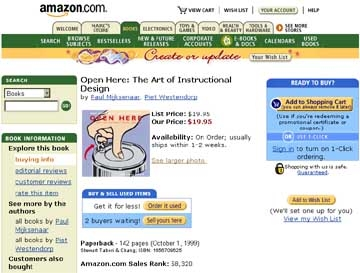
\includegraphics[width=\marginparwidth]{sample.jpg}
%%  \caption{A marginal figure.}
%%  \label{fig:marginparsample}
%%  \end{center}  
%%\end{figure}
%%}
%
%Aliquam consectetur quam sed odio varius vitae rhoncus urna fermentum. Phasellus viverra diam non justo porttitor varius. Integer ultrices accumsan lectus eget mollis. Nulla et leo sit amet nunc ornare rutrum sit amet ac dui. Cras vehicula accumsan purus nec fermentum. Mauris viverra condimentum metus, ut posuere quam laoreet nec. Phasellus massa tellus, ullamcorper nec porta sed, aliquet vitae nulla. Phasellus non tortor mauris. Cras ullamcorper egestas erat, vel rutrum elit viverra a. Donec in nisl ut est facilisis blandit. Quisque congue accumsan risus, ut venenatis magna vulputate vel. Nam commodo sapien vel mauris adipiscing nec dictum quam congue. Phasellus tempor vestibulum nisl quis blandit. Nullam condimentum auctor nibh, quis elementum libero tristique.



%\section{Acknowledgements}
%We thank all DUX 2003 publications support and staff who wrote this document originally and allowed us to modify it for this conference.
%This template was based on Manas Tungare's \texttt{chi.cls}, and rewritten by Luis A. Leiva.

\balance
\bibliographystyle{acm-sigchi}
\bibliography{pccworkshop}

\end{document}
